% Options for packages loaded elsewhere
\PassOptionsToPackage{unicode}{hyperref}
\PassOptionsToPackage{hyphens}{url}
%
\documentclass[
]{article}
\usepackage{lmodern}
\usepackage{amssymb,amsmath}
\usepackage{ifxetex,ifluatex}
\ifnum 0\ifxetex 1\fi\ifluatex 1\fi=0 % if pdftex
  \usepackage[T1]{fontenc}
  \usepackage[utf8]{inputenc}
  \usepackage{textcomp} % provide euro and other symbols
\else % if luatex or xetex
  \usepackage{unicode-math}
  \defaultfontfeatures{Scale=MatchLowercase}
  \defaultfontfeatures[\rmfamily]{Ligatures=TeX,Scale=1}
\fi
% Use upquote if available, for straight quotes in verbatim environments
\IfFileExists{upquote.sty}{\usepackage{upquote}}{}
\IfFileExists{microtype.sty}{% use microtype if available
  \usepackage[]{microtype}
  \UseMicrotypeSet[protrusion]{basicmath} % disable protrusion for tt fonts
}{}
\makeatletter
\@ifundefined{KOMAClassName}{% if non-KOMA class
  \IfFileExists{parskip.sty}{%
    \usepackage{parskip}
  }{% else
    \setlength{\parindent}{0pt}
    \setlength{\parskip}{6pt plus 2pt minus 1pt}}
}{% if KOMA class
  \KOMAoptions{parskip=half}}
\makeatother
\usepackage{xcolor}
\IfFileExists{xurl.sty}{\usepackage{xurl}}{} % add URL line breaks if available
\IfFileExists{bookmark.sty}{\usepackage{bookmark}}{\usepackage{hyperref}}
\hypersetup{
  hidelinks,
  pdfcreator={LaTeX via pandoc}}
\urlstyle{same} % disable monospaced font for URLs
\usepackage{graphicx,grffile}
\makeatletter
\def\maxwidth{\ifdim\Gin@nat@width>\linewidth\linewidth\else\Gin@nat@width\fi}
\def\maxheight{\ifdim\Gin@nat@height>\textheight\textheight\else\Gin@nat@height\fi}
\makeatother
% Scale images if necessary, so that they will not overflow the page
% margins by default, and it is still possible to overwrite the defaults
% using explicit options in \includegraphics[width, height, ...]{}
\setkeys{Gin}{width=\maxwidth,height=\maxheight,keepaspectratio}
% Set default figure placement to htbp
\makeatletter
\def\fps@figure{htbp}
\makeatother
\setlength{\emergencystretch}{3em} % prevent overfull lines
\providecommand{\tightlist}{%
  \setlength{\itemsep}{0pt}\setlength{\parskip}{0pt}}
\setcounter{secnumdepth}{-\maxdimen} % remove section numbering

\date{}

\begin{document}

実験データ解析演習 最終レポート

2610180082 2年1組 No. 39 水野 響

グループ番号:1

共同メンバー:藤浪真尋, 山崎大知

\hypertarget{header-n2003}{%
\section{テーマ}\label{header-n2003}}

主成分分析で天候に大きく寄与する成分を見つける
サポートベクターマシーンで新潟のお米の収量とその気候の関連性を調べる

\hypertarget{header-n2005}{%
\section{原理}\label{header-n2005}}

\hypertarget{header-n2006}{%
\subsubsection{主成分分析}\label{header-n2006}}

書くかぁ...

\hypertarget{header-n2009}{%
\subsubsection{サポートベクターマシン}\label{header-n2009}}

サポートベクターマシンでは,
自明に2群に線形分離可能である学習データを用いてその2群を最もよく分離する関数を考える.
個体あるいは対象を特徴づけるp個の変数
\(\textbf{x} = (x_1, x_2, \cdots., x_p)^T\) に関して観測されたn個の

\hypertarget{header-n2013}{%
\section{データ}\label{header-n2013}}

\hypertarget{header-n2014}{%
\subsubsection{米の収量}\label{header-n2014}}

\begin{itemize}
\item
  10aあたりの収量
\item
  出典:eStat
\end{itemize}

\hypertarget{header-n2019}{%
\subsubsection{天気}\label{header-n2019}}

\begin{itemize}
\item
  日照時間, 気温, 湿度, 降水量, 風速, 雲量
\item
  出典:気象庁
\end{itemize}

\hypertarget{header-n2026}{%
\section{手法}\label{header-n2026}}

\begin{enumerate}
\def\labelenumi{\arabic{enumi}.}
\item
  6次元の気候データを主成分分析により2次元に圧縮した.
\item
  収量を480 (t)以上の年を豊作とし, ラベルを豊作の年を1,
  不作の年を0としてラベル付けをした.
\item
  主成分分析した2次元データと固有ベクトルを月ごとにプロットした.
\item
  第一主成分と第二主成分の配列を用意した.
\item
  主成分をtrainデータとtestデータを7:3の割合で分割した.
\item
  サポートベクターマシーンを学習させた.
\item
  サポートベクターマシーンの正答率を求めた.
\item
  横軸を第一主成分, 縦軸を第二主成分としてデータをプロットし,
  サポートベクターマシーンの分類結果を可視化した.
\item
  以上を12ヶ月分同様に行った.
\item
  result配列を用意し,
  月ごとの第一主成分と第二主成分とサポートベクターマシーンの正答率を格納した.
\end{enumerate}

\hypertarget{header-n2048}{%
\section{結果}\label{header-n2048}}

操作による散布図が図1である. 操作による散布図が図2である.

月ごとの第一主成分と第二主成分とサポートベクターマシーンの正答率が表hugaである.

\begin{figure}
\centering
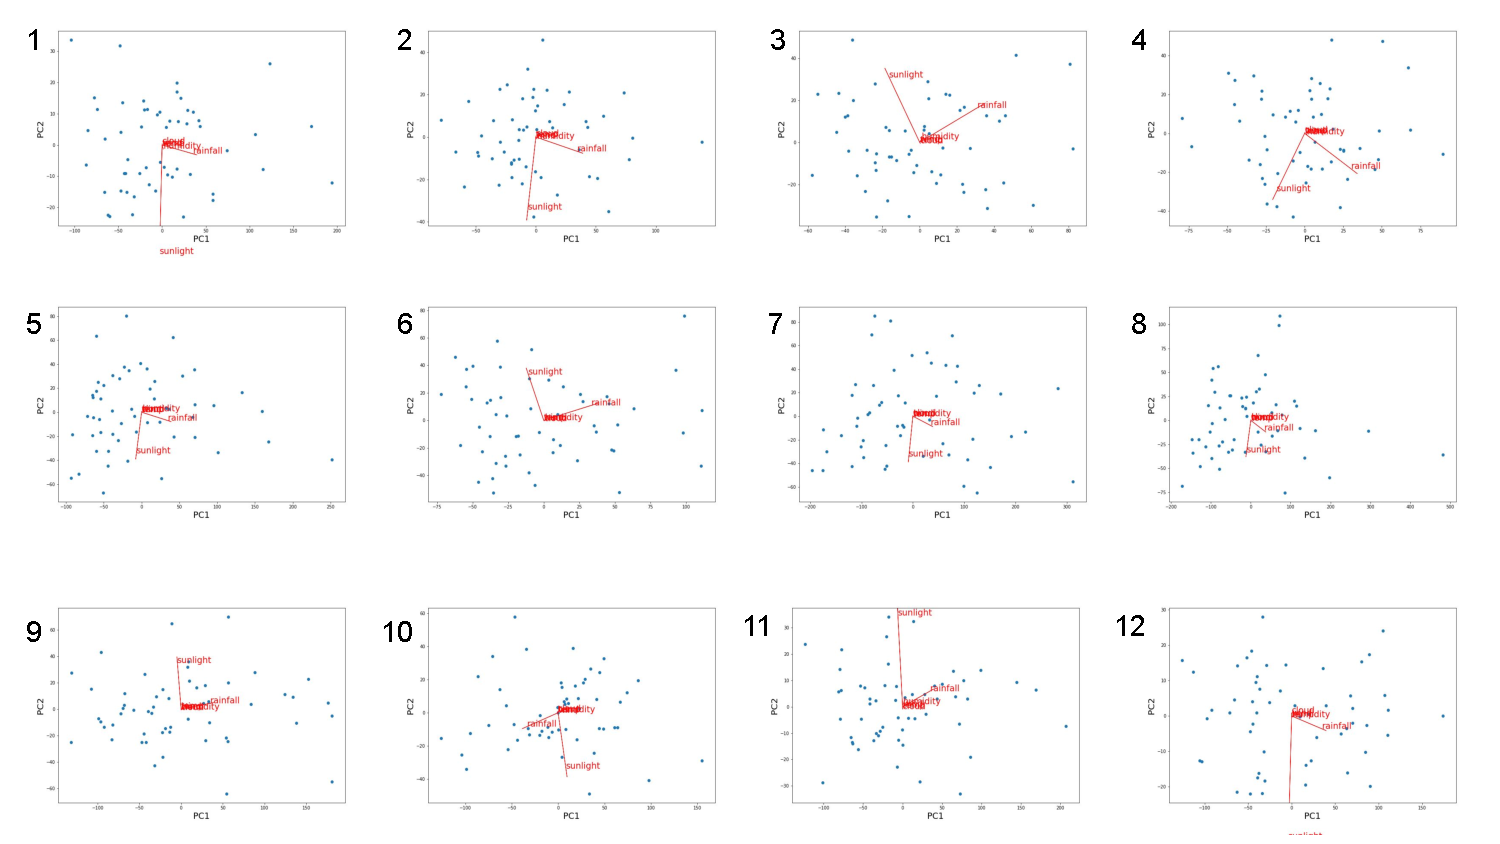
\includegraphics{/Users/ev180082/experiment_data_parsing_exercise/100tweet/pca_plot.pdf}
\caption{PCAによる分析結果}
\end{figure}

\begin{figure}
\centering
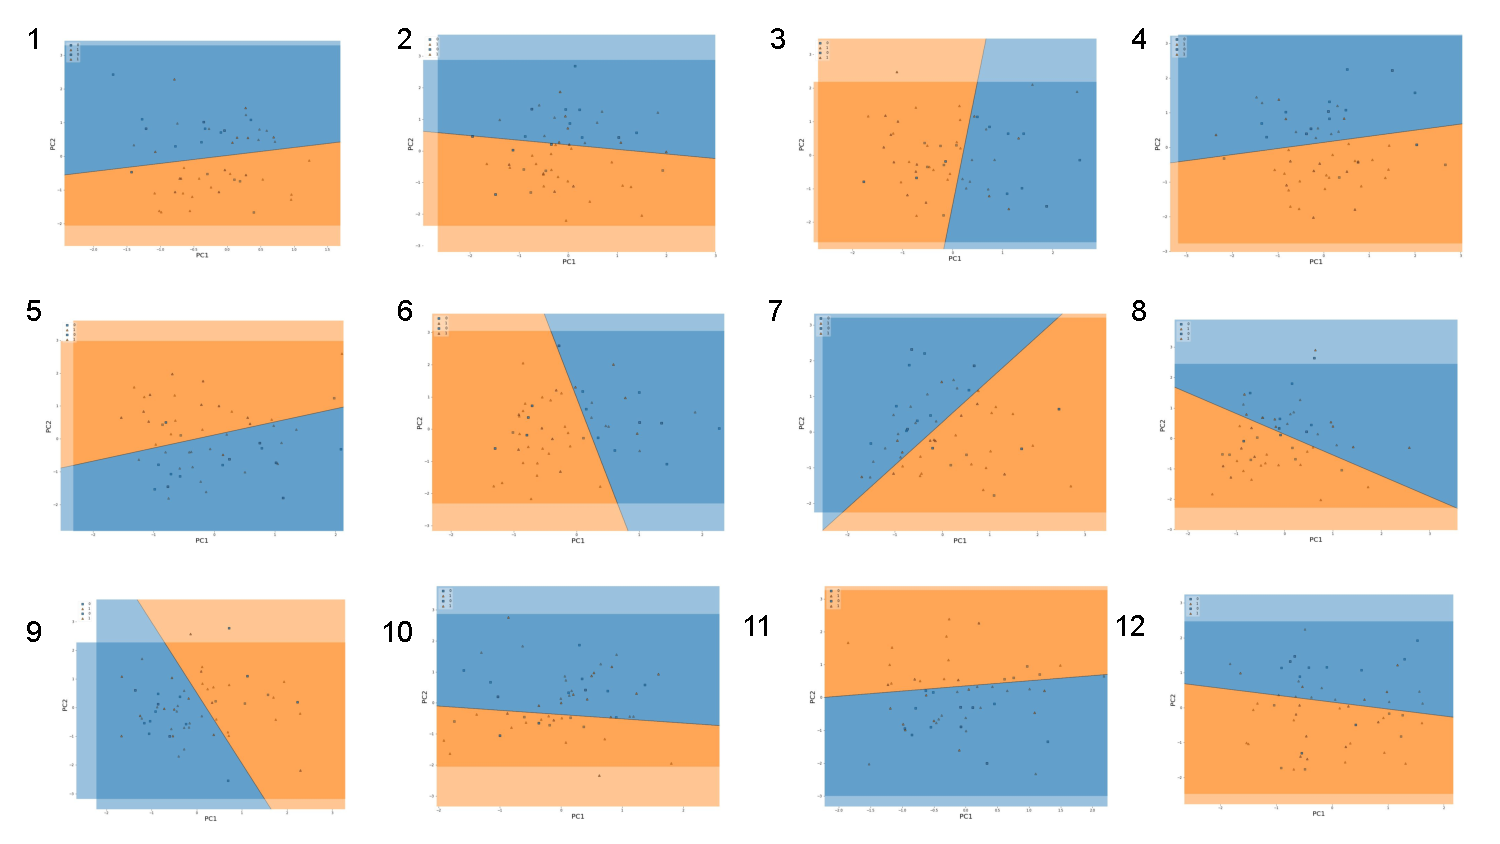
\includegraphics{/Users/ev180082/experiment_data_parsing_exercise/100tweet/svm_plot.pdf}
\caption{SVMによる分析結果}
\end{figure}

\begin{verbatim}
             PC1       PC2  SVM_score
 month                               
 1      0.948290  0.049088   0.529412
 2      0.841302  0.151448   0.352941
 3      0.726571  0.266117   0.588235
 4      0.707992  0.285218   0.705882
 5      0.718615  0.278711   0.882353
 6      0.835200  0.163343   0.529412
 7      0.907491  0.091873   0.588235
 8      0.902660  0.096692   0.352941
 9      0.906668  0.092054   0.3520961
 10     0.867753  0.129710   0.235294
 11     0.953945  0.043966   0.470588
 12     0.965803  0.031950   0.5882
\end{verbatim}

\hypertarget{header-n2056}{%
\section{考察}\label{header-n2056}}

第二主成分の寄与率が高い月はSVMの正答率が高い。特に5月はSVMの正答率が高い。それら以外はあてになる分析結果とはいえない。

固有ベクトルから、4月5月は日照時間が多い方が良いと考えられる。

データをもっとよく観察して、ある程度仮説を立てるべきだった。

\end{document}
